%Version 2.1 April 2023
% See section 11 of the User Manual for version history
%
%%%%%%%%%%%%%%%%%%%%%%%%%%%%%%%%%%%%%%%%%%%%%%%%%%%%%%%%%%%%%%%%%%%%%%
%%                                                                 %%
%% Please do not use \input{...} to include other tex files.       %%
%% Submit your LaTeX manuscript as one .tex document.              %%
%%                                                                 %%
%% All additional figures and files should be attached             %%
%% separately and not embedded in the \TeX\ document itself.       %%
%%                                                                 %%
%%%%%%%%%%%%%%%%%%%%%%%%%%%%%%%%%%%%%%%%%%%%%%%%%%%%%%%%%%%%%%%%%%%%%

\documentclass[sn-basic,pdflatex]{sn-jnl}

%%%% Standard Packages
%%<additional latex packages if required can be included here>

\usepackage{graphicx}%
\usepackage{multirow}%
\usepackage{amsmath,amssymb,amsfonts}%
\usepackage{amsthm}%
\usepackage{mathrsfs}%
\usepackage[title]{appendix}%
\usepackage{xcolor}%
\usepackage{textcomp}%
\usepackage{manyfoot}%
\usepackage{booktabs}%
\usepackage{algorithm}%
\usepackage{algorithmicx}%
\usepackage{algpseudocode}%
\usepackage{listings}%
%%%%

%%%%%=============================================================================%%%%
%%%%  Remarks: This template is provided to aid authors with the preparation
%%%%  of original research articles intended for submission to journals published
%%%%  by Springer Nature. The guidance has been prepared in partnership with
%%%%  production teams to conform to Springer Nature technical requirements.
%%%%  Editorial and presentation requirements differ among journal portfolios and
%%%%  research disciplines. You may find sections in this template are irrelevant
%%%%  to your work and are empowered to omit any such section if allowed by the
%%%%  journal you intend to submit to. The submission guidelines and policies
%%%%  of the journal take precedence. A detailed User Manual is available in the
%%%%  template package for technical guidance.
%%%%%=============================================================================%%%%

%% Per the spinger doc, new theorem styles can be included using built in style, 
%% but it seems the don't work so commented below
%\theoremstyle{thmstyleone}%
\newtheorem{theorem}{Theorem}%  meant for continuous numbers
%%\newtheorem{theorem}{Theorem}[section]% meant for sectionwise numbers
%% optional argument [theorem] produces theorem numbering sequence instead of independent numbers for Proposition
\newtheorem{proposition}[theorem]{Proposition}%
%%\newtheorem{proposition}{Proposition}% to get separate numbers for theorem and proposition etc.

%% \theoremstyle{thmstyletwo}%
\theoremstyle{remark}
\newtheorem{example}{Example}%
\newtheorem{remark}{Remark}%

%% \theoremstyle{thmstylethree}%
\theoremstyle{definition}
\newtheorem{definition}{Definition}%



\raggedbottom




% tightlist command for lists without linebreak
\providecommand{\tightlist}{%
  \setlength{\itemsep}{0pt}\setlength{\parskip}{0pt}}





\begin{document}


\title[Lab Notebook]{Ordinal Pattern Analysis for Early Bearing Fault
Detection and Classification in Rotating Machinery}

%%=============================================================%%
%% Prefix	-> \pfx{Dr}
%% GivenName	-> \fnm{Joergen W.}
%% Particle	-> \spfx{van der} -> surname prefix
%% FamilyName	-> \sur{Ploeg}
%% Suffix	-> \sfx{IV}
%% NatureName	-> \tanm{Poet Laureate} -> Title after name
%% Degrees	-> \dgr{MSc, PhD}
%% \author*[1,2]{\pfx{Dr} \fnm{Joergen W.} \spfx{van der} \sur{Ploeg} \sfx{IV} \tanm{Poet Laureate}
%%                 \dgr{MSc, PhD}}\email{iauthor@gmail.com}
%%=============================================================%%

\author*[1]{\fnm{Rasika} \sur{Dilhani} \dgr{PhD}}\email{\href{mailto:rasidilhani@gmail.com}{\nolinkurl{rasidilhani@gmail.com}}}

\author[1]{\fnm{Alejandro} \sur{Author} }



  \affil*[1]{\orgdiv{School of Mathematics and
Statistics}, \orgname{Victoria University of
Wellington}, \orgaddress{\city{Wellington}, \country{New
Zealand}, \postcode{6012}, \state{}, \street{}}}

\abstract{The purpose of this research is to identify perturbation
machines from the time series data. Chaos are hard to detect from time
series. Bandt and Pompe proposed looking at time series from the
perspective of ordinal patterns to develop fast and automated methods
for extracting qualitative information from nonlinear time series. They
developed the idea of permutation entropy to measure the complexity of a
system underlying a time series, taking into account the ordinal
patterns that represent the variations in a time series. Only one aspect
of the ordinal structure of a time series is revealed by the permutation
entropy. Here we show how to use the real-valued data set to extract all
ordinal information.}

\keywords{ordinal patterns, permutation entropy, bearing fault data}



\maketitle

\section{Introduction}\label{sec1}

Bearings are critical components in rotating machinery, yet their
demanding operating conditions involving high loads and impacts often
lead to various faults. These faults can result in significant downtime,
costly maintenance, and even complete machine failure. Therefore, early
and accurate detection and classification of bearing faults are
essential for ensuring operational reliability and minimizing
maintenance expenses.

Traditional fault detection methods primarily rely on analyzing physical
parameters and trends using techniques such as vibration analysis,
thermal monitoring, and current signature analysis. While these methods
have proven effective, they can be susceptible to noise and often
require substantial computational resources. Ordinal pattern analysis
has emerged as a promising alternative, offering a robust and
computationally efficient approach for analyzing time series data.

At its core, ordinal pattern analysis involves transforming continuous
time series data into a sequence of ordinal patterns that represent the
order relationships among data points within a given time window. This
approach effectively captures the fundamental dynamics of the signal in
a manner that is inherently robust to noise and distortions. By
analyzing these patterns, it becomes possible to identify subtle changes
in system behavior that may indicate the presence of a fault.

This study investigates the application of ordinal pattern analysis for
early detection and classification of bearing faults, focusing on common
fault types such as ball, outer race, and inner race defects. Using a
publicly available dataset from the Case Western Reserve University
Bearing Data Center, we will demonstrate the effectiveness of ordinal
patterns in distinguishing between healthy and faulty bearing
conditions.

Our research will explore the advantages of ordinal pattern analysis in
detecting changes in system dynamics associated with faults. By
identifying alterations in the frequency and recurrence of specific
temporal patterns, this technique can reveal subtle indicators of
developing faults. Furthermore, unlike some traditional methods limited
to linear systems, ordinal pattern analysis can effectively detect
faults in complex, non-linear systems, broadening its applicability.

Traditional methods often rely on specialized sensors and data
acquisition systems, ordinal pattern analysis can potentially achieve
comparable results using simpler time series data, highlighting its
potential for wider adoption. We will investigate the sensitivity of
ordinal pattern analysis to subtle changes in system dynamics,
particularly within complex systems, where its strengths may be most
pronounced.

We aim to establish ordinal pattern analysis as a viable and
advantageous tool for bearing fault diagnosis, contributing to the
advancement of predictive maintenance technologies and promoting more
efficient and reliable operation of rotating machinery.

\section{Literature Review}\label{sec2}

In the study conducted by researchers \citet{WOS:000312724900101}, an
enhanced approach is introduced to detect bearing faults through the
utilization of high-frequency resonance, resulting in improved precision
and dependability in diagnosing faults within mechanical systems. The
investigation illustrates that this refined methodology adeptly
recognizes initial bearing abnormalities, representing a significant
progression compared to conventional diagnostic techniques. The article
by \citet{WOS:000301688000008} presents a new technique for fault
identification which employs an adaptive rank-order morphological filter
to categorize patterns in one-dimensional signals. This strategy
enhances the precision and resilience of fault diagnosis by proficiently
sifting through and pinpointing signal irregularities. Furthermore,
\citet{WOS:000303039300034} propose an approach for early fault
detection in machinery by scrutinizing truncated vibration signals using
Shannon wavelet spectrum analysis. This method heightens the detection
of emerging faults, thereby enhancing the prognostic maintenance of
equipment.

\citet{WOS:000345844100102} discusses a prototype FPGA implementation
that uses machine learning to convert analog signals into concise
feature representations. It employs an event-based methodology to
enhance the efficiency and accuracy of signal processing across various
applications. \citet{WOS:000396580800080} discusses the utilization of a
dedicated hierarchy of neural networks for evaluating bearing
degradation, thereby enhancing the precision and dependability of
diagnosing the state and remaining operational life of bearings in
machinery. By amalgamating multifractal detrended fluctuation analysis
with the Mahalanobis distance criterion \citep{WOS:000320835800016}, the
research in the publication enhances the fault diagnosis of rolling
bearings, leading to improved diagnostic accuracy and offering
efficient, validated approaches for early fault detection in industrial
settings.

An additional intriguing research study detailed in the publication
\citet{WOS:000360994300029} introduces a diagnostic technique for
rolling element bearings grounded in the concept of active perception.
This method revolves around examining the dynamic interactions between
the bearing and its surroundings. Noteworthy discoveries include the
capability of the approach to precisely evaluate the bearing's condition
by integrating perceptual cues and responses, thereby enhancing fault
detection and predictive maintenance strategies.
\citet{WOS:000343577703075} presents a fault diagnosis approach for
rolling element bearings that makes use of Empirical Mode Decomposition
(EMD) in conjunction with Discrete Fourier Domain Analysis (DFDA). This
technique proficiently isolates and scrutinizes fault-related
characteristics in vibration signals, resulting in enhanced accuracy and
dependability in the diagnosis of bearing conditions. The utilization of
a signal-based triangular structuring element for mathematical
morphological analysis, along with the application of this method to
boost fault diagnosis in rolling element bearings through the effective
processing and interpretation of vibration signal features, was
deliberated in the publication \citep{WOS:000334316700001}. Furthermore,
a hybrid CEEMD-EMD strategy for fault detection in rolling bearings,
which merges Complete Ensemble Empirical Mode Decomposition with Noise
(CEEMD) and traditional Empirical Mode Decomposition (EMD) to enhance
the precision of vibration signal analysis and augment fault detection
capabilities, has been enhanced in the manuscript
\citet{WOS:000412752200052}.

The authors of the paper \citet{WOS:000335959500009} propose a
methodology for bearing fault detection that utilizes compressive
measurements of vibration signals to efficiently detect faults,
enhancing diagnostic accuracy while reducing the data processing load. A
unique technique for feature extraction, based on the crossover
characteristics of nonlinear data, is applied to enhance fault diagnosis
in rotary machinery by effectively identifying critical patterns in
complex signal data \citep{WOS:000338603900013}. Self-Organizing Maps
(SOMs) are successful in diagnosing motor bearing faults through the
classification of complex vibration data, while approaches based on fast
nonlocal means and envelope spectra contribute to improving fault
diagnosis accuracy. Moreover, a low-dimensional compressed measurement
strategy boosts fault detection efficiency, and a Bayesian inference
technique guided by a smoothness index enables precise identification of
various bearing faults by analyzing anti-symmetric real Laplace wavelet
parameters
\citep{WOS:000380543400119, WOS:000348309400067, WOS:000354607100016, WOS:000350998800016}.
A novel machine fault diagnosis method using the Statistical Local
Linear Embedding Algorithm (S-LLE), an LLE extension leveraging fault
class labels to enhance feature extraction, dimensionality reduction,
and pattern recognition by mapping high-dimensional vibration signal
vectors---processed through time-domain, frequency-domain, and empirical
mode decomposition (EMD)---into a low-dimensional space, which
outperforms PCA, LDA, and LLE for swift fault classification, as
validated by rolling bearing error signals, thereby achieving superior
error classification performance over conventional methods
\citep{WOS:000361788200068}. The combination of wavelet packet
decomposition with multi-scale permutation entropy exhibits potential in
accurately detecting bearing faults, utilizing hidden Markov models
\citep{WOS:000362513400031}. Results demonstrate that this approach
significantly improves fault detection accuracy compared to traditional
methods, achieving higher precision in identifying fault types and their
severity. Integrating wavelet packet decomposition with multi-scale
permutation entropy enhances the reliability of fault diagnosis systems,
making it a valuable technique for predictive maintenance in industrial
applications.

\citet{WOS:000365686400021} introduce a new feature extraction technique
called Window Marginal Spectrum Clustering (WMSC) for diagnosing faults
in roller element bearings (REBs). This method utilizes the
Hilbert-Huang Transform (HHT) and Support Vector Machines (SVM) to
improve classification accuracy and robustness against Gaussian white
noise. Experimental results with datasets from the Bearing Data Center
of Case Western Reserve University (CWRU) demonstrate that WMSC
outperforms conventional methods. \citet{WOS:000366534900022} presents
``The Diagnostic Line,'' a novel criterion for monitoring the condition
of rotating machinery. This approach aims to enhance the accuracy and
reliability of machinery health diagnosis. A comparative analysis, using
data from Case Western Reserve University, was conducted to evaluate
various diagnostic techniques and establish a standard reference for
bearing fault diagnosis \citep{WOS:000357230900007}.
\citet{WOS:000385104500001} proposes an improved Wavelet Total Variation
Denoising (W-TVD) technique for mechanical fault diagnosis, effectively
filtering noise and enhancing fault detection accuracy, with findings
showing that this approach significantly outperforms traditional
denoising methods in diagnostic performance. The research on fault
diagnosis in industrial rotating equipment using permutation entropy,
signal processing techniques, and a multi-output neuro-fuzzy classifier
demonstrates effective identification of fault types and severity
levels. The results show that combining permutation entropy for feature
extraction with signal processing improves the clarity and distinction
of fault signatures, while the neuro-fuzzy classifier achieves high
accuracy in multi-class fault identification. The study concludes that
this integrated approach enhances diagnostic reliability and
performance, making it a robust solution for real-time fault detection
in industrial machinery \citep{Rajabi2022}. An adapted kernel marginal
Fisher analysis (MKMFA) technique for feature extraction and
dimensionality reduction to enhance bearing fault diagnosis accuracy is
elaborated in a study; by extracting critical low-dimensional features
and employing a K-nearest neighbor classifier, it exhibits superior
performance in comparison to alternative approaches when utilized for
identifying diverse bearing faults \citep{WOS:000392016300001}.

Signal analysis of vibrations is a significantly efficient approach for
diagnosing mechanical faults. However, the identification of defects in
their early stages poses a challenge due to the presence of noise from
components \citep{WOS:000369301600001, WOS:000367992900001}. These
studies introduce a fresh methodology that merges time domain analysis
with adaptive fuzzy C-means clustering. \citet{WOS:000366765500038}
introduces an innovative technique for assessing machinery damage,
utilizing manifold learning principles to compute subspace distances.
\citet{WOS:000379556300014} presents the utilization of Multivariate
Empirical Mode Decomposition (MEMD) in diagnosing rolling bearings'
faults. It demonstrates the effectiveness of this method in improving
fault detection by thoroughly analyzing complex, multidimensional signal
data. \citet{WOS:000391229300006} proposes a methodology for diagnosing
faults in rolling element bearings by integrating Multifractal Theory
and Gray Relation Theory. This integration is designed to improve the
precision and reliability of fault detection and analysis, ultimately
enhancing diagnostic results. A new approach for examining vibration
signals in rolling bearings, which combines dual-entropy, Holder
coefficient, and Gray Relation Theory is studied by
\citet{WOS:000426819400027}. This integration aims to improve the
efficiency of fault detection and analysis by leveraging these methods
to achieve higher levels of precision and reliability in diagnostics.

\citet{WOS:000398818700108} discusses the Shock Pulse Index (SPI) and
its application in diagnosing faults in rolling element bearings,
highlighting SPI's effectiveness in detecting and analyzing bearing
condition and performance issues. The results demonstrate that SPI
provides accurate fault detection and is a valuable tool for monitoring
and diagnosing bearing health. Fault diagnosis for rolling bearings
under variable conditions using visual cognition techniques is discusses
by \citet{WOS:000404415000016}. Results indicate that visual cognition
methods significantly improve the ability to identify and assess bearing
faults in changing operational environments. The paper by
\citet{WOS:000401109400020} introduces sparse discriminant manifold
projections for bearing fault diagnosis, leveraging advanced
dimensionality reduction techniques to enhance fault detection and
classification accuracy. Results show that this method effectively
identifies bearing faults by capturing essential discriminative features
while reducing noise and irrelevant data. \citet{WOS:000419006900041}
presents a fault detection method for rolling bearings' vibration
signals using the Symplectic Entropy method, which analyzes the
complexity and patterns of vibration data to improve fault
identification accuracy. Results demonstrate that this approach
effectively detects faults by providing a robust measure of signal
irregularities and anomalies. A method for extracting incipient fault
features in rolling bearings using an autocorrelation function impulse
harmonic-to-noise ratio index, combined with Singular Value
Decomposition (SVD) and the Teager Energy Operator; results show that
this approach effectively identifies early-stage faults by enhancing the
detection of subtle signal anomalies amidst noise
\citep{WOS:000416794600016}. \citet{WOS:000484465800028} present a
bearing fault diagnosis method that combines autoencoders with Particle
Swarm Optimization (PSO) and Support Vector Machines (SVM); this
approach leverages autoencoders for feature extraction and
dimensionality reduction, while PSO optimizes the SVM parameters,
resulting in improved diagnostic accuracy and robustness in identifying
bearing faults. An optimized resolution coefficient algorithm for the
Gray Relation Classifier, aiming to enhance classification accuracy by
improving the algorithm's ability to distinguish between different
classes through refined resolution coefficients, leading to more precise
fault diagnosis and analysis \citep{WOS:000477760600037}.
\citet{WOS:000477760600061} proposes a signal subtle feature extraction
algorithm using an improved fractal box-counting dimension method, which
enhances the detection of fine-grained features in signals by refining
the fractal dimension calculation, resulting in better identification
and analysis of subtle signal patterns.

A novel rolling bearing fault detection method based on the Empirical
Wavelet Transform (EWT) effectively decomposes vibration signals into
components that emphasize fault-related features, thereby improving
detection accuracy and robustness in identifying bearing faults
\citep{WOS:000467079500501}. A bearing fault detection method has been
introduced by \citet{WOS:000459864800144} that combines Empirical Mode
Decomposition (EMD) with Random Forest effectively analyzes vibration
signals under varying operational conditions by decomposing them into
intrinsic mode functions and classifying fault patterns, resulting in
enhanced detection accuracy and reliability. \citet{WOS:000458657500187}
critically examines the significance of feature extraction and selection
in diagnosing bearing defects, emphasizing that effective feature
extraction and selection are crucial for improving diagnostic accuracy
and reliability by identifying the most relevant characteristics from
vibration signals.

An online health status estimation technique for rolling bearings based
on vibration signals, with a focus on real-time monitoring and analysis
for evaluating bearing condition. It is shown in the research that this
method effectively assesses health status through continuous evaluation
of vibration data to identify and predict potential faults
\citep{WOS:000452922000015}. An automatic classification approach for
bearing faults is presented by \citet{WOS:000453413600001}, utilizing
deep learning methods that employ neural networks to examine and
categorize fault patterns present in vibration signals. This leads to
enhanced accuracy and efficiency in the detection and diagnosis of
bearing faults. \citet{WOS:000452819600235} introduces a method for
early fault diagnosis in bearings using Empirical Wavelet Transform
(EWT) in conjunction with energy entropy. By analyzing vibration signals
with detailed frequency decomposition and measuring the distribution of
signal energy, this method improves the identification accuracy of early
faults. Another study \citet{WOS:000450745100001} and
\citet{WOS:000449334500118} introduces a technique for detecting faults
in rolling element bearings that involves segmenting vibration signals
and applying wavelet analysis and deep neural networks. This method
improves fault detection by segmenting the signal into meaningful parts
for better accuracy, utilizing wavelet transforms for extracting
features, and employing deep neural networks for clustering and
categorizing, resulting in more precise identification of bearing
faults.

The present study of \citet{WOS:000440977000032} introduces a technique
for extracting bearing fault features using autoregressive coefficients,
Linear Discriminant Analysis (LDA), and Support Vector Machines (SVM) in
varying operational conditions. These methods are combined to improve
fault detection by accurately identifying and categorizing fault
features even amidst changing operational settings. A unique diagnostic
approach for rolling element bearings is proposed, which integrates
Noise-Assisted Multivariate Empirical Mode Decomposition (MEMD) with a
Functional Neural Fuzzy Network \citep{WOS:000434717400001}. This
integration utilizes MEMD to extract features effectively and the neural
fuzzy network for precise fault classification, resulting in enhanced
diagnostic precision and reliability. \citet{WOS:000426284100001}
presents a fault diagnosis method for rolling bearings that utilizes
Modified Local Fisher Discriminant Analysis (LFDA) and Empirical Mode
Decomposition (EMD) along with sensitive feature selection. The
objective is to enhance fault detection by extracting and examining
critical features from vibration signals with improved accuracy and
discrimination. \citet{WOS:000539546400083} details an initial fault
diagnosis technique for rolling bearings that merges Empirical Wavelet
Transform (EWT) with Spectral Kurtosis. The focus is on detecting
initial faults through refined frequency analysis with EWT and
highlighting abnormal signal features using Spectral Kurtosis, leading
to improved early fault detection and diagnostic accuracy. Another study
of \citet{hakim2023systematic} introduces an enhanced similarity-based
modeling approach for classifying failures in rotating machines. By
utilizing advanced similarity measures to better match failure patterns
and improve diagnostic precision, the accuracy and effectiveness of
fault classification are significantly enhanced. Results indicate that
this approach surpasses traditional classification techniques, achieving
higher accuracy and reliability in failure detection. A comprehensive
review is provided on fault diagnosis methods for rolling bearings that
employ deep learning and transfer learning.

\citet{WOS:000345844100102} discusses a prototype FPGA implementation
that uses machine learning to convert analog signals into concise
feature representations. It employs an event-based methodology to
enhance the efficiency and accuracy of signal processing across various
applications. \citet{WOS:000396580800080} explores a dedicated hierarchy
of neural networks to assess bearing degradation, aiming to improve the
accuracy and reliability of diagnosing machinery bearing conditions and
estimating their remaining operational life. By amalgamating
multifractal detrended fluctuation analysis with the Mahalanobis
distance criterion, the research in the publication enhances the fault
diagnosis of rolling bearings, leading to improved diagnostic accuracy
and offers efficient, validated approaches for early fault detection in
industrial settings \citep{WOS:000320835800016}.

An additional intriguing research study detailed in
\citet{WOS:000360994300029} introduces a diagnostic technique for
rolling element bearings grounded in the concept of active perception.
This method revolves around examining the dynamic interactions between
the bearing and its surroundings. Noteworthy discoveries include the
capability of the approach to precisely evaluate the bearing's condition
by integrating perceptual cues and responses, thereby enhancing fault
detection and predictive maintenance strategies. The study described in
\citet{WOS:000343577703075} presents a fault diagnosis approach for
rolling element bearings that makes use of Empirical Mode Decomposition
(EMD) in conjunction with Discrete Fourier Domain Analysis (DFDA). This
technique proficiently isolates and scrutinizes fault-related
characteristics in vibration signals, resulting in enhanced accuracy and
dependability in the diagnosis of bearing conditions. The utilization of
a signal-based triangular structuring element for mathematical
morphological analysis, along with the application of this method to
boost fault diagnosis in rolling element bearings through the effective
processing and interpretation of vibration signal features, was
deliberated in the publication \citet{WOS:000334316700001}. Furthermore,
a hybrid CEEMD-EMD strategy for fault detection in rolling bearings,
which merges Complete Ensemble Empirical Mode Decomposition with Noise
(CEEMD) and traditional Empirical Mode Decomposition (EMD) to enhance
the precision of vibration signal analysis and augment fault detection
capabilities, has been enhanced in the manuscript
\citet{WOS:000412752200052}.

\citet{WOS:000335959500009} propose a methodology for bearing fault
detection that utilizes comprehensive measurements of vibration signals
to efficiently detect faults, thereby enhancing diagnostic accuracy
while reducing the data processing load. A unique feature extraction
technique based on the crossover properties of nonlinear data is applied
to improve fault diagnosis in rotating machinery by effectively
identifying critical patterns in complex signal data
\citep{WOS:000338603900013}. Research studies show that self-organizing
maps (SOMs) are successful in diagnosing engine bearing faults by
classifying complex vibration data, while approaches based on fast
non-local averages and envelope spectra help improve fault diagnosis
accuracy. In addition, a low-dimensional compressed measurement strategy
increases the error detection efficiency, and a Bayesian inference
technique based on a smoothness index enables the precise identification
of various bearing errors through the analysis of anti symmetric real
Laplace wavelet parameters
\citep{WOS:000380543400119, WOS:000348309400067, WOS:000354607100016, WOS:000350998800016}.
Recent scholarly investigations have concentrated on advanced
methodologies for bearing fault diagnosis using vibration signals.
Statistical locally linear embedding has been suggested as a potent
technique for dimensional reduction and feature extraction, surpassing
conventional methods like PCA and LDA \citep{WOS:000361788200068}. The
combination of wavelet packet decomposition with multi-scale permutation
entropy exhibits potential in accurately detecting bearing faults
utilizing hidden Markov models \citep{WOS:000362513400031}. Results
demonstrate that this approach significantly improves fault detection
accuracy compared to traditional methods, achieving higher precision in
identifying fault types and their severity. Integrating wavelet packet
decomposition with multi-scale permutation entropy enhances the
reliability of fault diagnosis systems, making it a valuable technique
for predictive maintenance in industrial applications.

\citet{WOS:000365686400021} introduces a new feature extraction
technique called Window Marginal Spectrum Clustering (WMSC) for
diagnosing faults in roller element bearings (REBs). This method
utilizes the Hilbert-Huang Transform (HHT) and Support Vector Machines
(SVM) to improve classification accuracy and robustness against Gaussian
white noise. Experimental results with data sets from the Bearing Data
Center of Case Western Reserve University (CWRU) demonstrate that WMSC
outperforms conventional methods. Additionally,
\citet{WOS:000366534900022} presents ``The Diagnostic Line,'' a novel
criterion for monitoring the condition of rotating machinery. This
approach aims to enhance the accuracy and reliability of machinery
health diagnosis. Another comparative analysis, using data from Case
Western Reserve University, was conducted to evaluate various diagnostic
techniques and establish a standard reference for bearing fault
diagnosis \citep{WOS:000357230900007}. The current study is built upon
this investigation, incorporating the same data set for further
examination employing a novel time series model.

Furthermore, an innovative two-stage strategy is developed that utilizes
permutation entropy for fault detection along with wavelet packet
transform, envelope analysis and neuro-fuzzy classification for fault
isolation, demonstrating improved diagnostic performance compared to
existing techniques \citep{WOS:000385104500001, Rajabi2022}. These
advances contribute to more precise and effective bearing fault
diagnosis in rotating industrial machines. A study elaborates an adapted
kernel marginal Fisher analysis (MKMFA) technique for feature extraction
and dimensionality reduction to improve the accuracy of bearing fault
diagnosis. By extracting critical low-dimensional features and using a
K-nearest neighbor classifier, it exhibits superior performance compared
to alternative approaches when used to identify various bearing defects
\citep{WOS:000392016300001}.

Vibration signal analysis is an extremely efficient approach to
diagnosing mechanical faults. However, identifying early-stage defects
is challenging due to component noise
\citep{WOS:000369301600001, WOS:000367992900001}. This study presents a
new methodology that combines time domain analysis with adaptive fuzzy
C-means clustering. It uses nine standard parameters in the time domain
to construct characteristic vectors and improves clustering by
optimizing with five specific parameters (such as variance, RMS,
kurtosis, skewness and crest factor). Research shows the ability to
detect errors sensitively, even for minor errors. In addition, an
innovative fault diagnosis technique for rolling bearings is developed
by integrating the Multifractal Detrended Fluctuation Analysis (MFDFA)
and Alpha Stable Distribution (ASD) functions.

The article by \citet{WOS:000366765500038} presents an innovative
technique for assessing machine damage that uses a variety of learning
principles to calculate subspace distances. This method improves the
accuracy and responsiveness of damage assessment by applying advanced
dimensionality reduction techniques. \citet{WOS:000379556300014}
presents the use of Multivariate Empirical Mode Decomposition (MEMD) in
the diagnosis of rolling bearing defects. It demonstrates the
effectiveness of this method in improving fault detection through
in-depth analysis of complex, multi-dimensional signal data. The
manuscript \citet{WOS:000391229300006} proposes a methodology for
diagnosing defects in rolling bearings by integrating multifractal
theory and Gray relations theory. This integration is intended to
improve the precision and reliability of fault detection and analysis
and ultimately improve diagnostic results. The study presents a new
approach to investigate vibration signals in rolling bearings that
combines dual entropy, Holder coefficient and Gray relations theory
\citep{WOS:000426819400027}. This integration aims to improve the
efficiency of fault detection and analysis by leveraging these methods
to achieve higher levels of precision and reliability in diagnosis.

\citet{WOS:000398818700108} discusses the Shock Pulse Index (SPI) and
its application in diagnosing failures in rolling bearings and
highlights the effectiveness of SPI in detecting and analyzing bearing
health and performance problems. The results show that SPI enables
accurate fault detection and is a valuable tool for monitoring and
diagnosing bearing condition. The present study discusses the diagnosis
of rolling bearing faults under variable conditions using visual
detection techniques. The objective is to demonstrate how visual
analysis can enhance the accuracy of fault detection and diagnosis. The
findings indicate that visual detection methods markedly enhance the
capacity to identify and assess bearing defects in dynamic operational
environments \citep{WOS:000404415000016}. \citet{WOS:000401109400020}
introduces sparse discriminant manifold projections for bearing fault
diagnosis and leverages advanced dimensionality reduction techniques to
improve fault detection and classification accuracy. The results show
that this method effectively identifies bearing defects by capturing key
distinguishing features while reducing noise and irrelevant data. In a
further study, \citet{WOS:000419006900041} presents a fault detection
method for rolling bearing vibration signals based on the symplectic
entropy method. This method analyses the complexity and patterns of
vibration data in order to improve the accuracy of fault detection. The
results demonstrate that this approach is an effective means of
detecting errors, providing a robust measure of signal irregularities
and anomalies.

A method for extracting incipient fault features in rolling bearings
using an autocorrelation function impulse harmonic noise ratio index
combined with Singular Value Decomposition (SVD) and the Teager Energy
Operator. The results show that this approach effectively identifies
early-stage errors by improving the detection of subtle signal anomalies
amid noise \citep{WOS:000416794600016}. \citet{WOS:000484465800028}
presents a method for bearing fault diagnosis that combines automatic
encoders with particle swarm optimization (PSO) and support vector
machines (SVM). This approach uses autoencoders for feature extraction
and dimensionality reduction, while PSO optimizes the SVM parameters,
resulting in improved diagnostic accuracy and robustness in bearing
fault identification. The paper presents an optimized resolution
coefficient algorithm for the Gray relation classifier, which aims to
improve classification accuracy by improving the algorithm's ability to
distinguish between different classes through refined resolution
coefficients, resulting in more precise fault diagnosis and -analysis
leads \citep{WOS:000477760600037}. \citet{WOS:000477760600061} proposes
an algorithm for extracting subtle signal features using an improved
fractal box counting dimension method, which improves the detection of
fine-grained features in signals by refining the fractal dimension
calculation, resulting in better identification and analysis of subtle
signal patterns.

A novel rolling bearing defect detection method based on empirical
wavelet transform (EWT), which effectively decomposes vibration signals
into components that highlight defect-related features, thereby
improving detection accuracy and robustness in bearing defect
identification \citep{WOS:000467079500501}. A bearing fault detection
method from \citet{WOS:000459864800144} that combines Empirical Mode
Decomposition (EMD) with Random Forest, which effectively analyzes
vibration signals under different operating conditions by decomposing
them into intrinsic mode functions and classifying fault patterns,
resulting in improved detection accuracy leads and reliability.
\citet{WOS:000458657500187} critically examines the importance of
feature extraction and selection in the diagnosis of bearing defects and
emphasizes that effective feature extraction and selection is crucial
for improving diagnostic accuracy and reliability by identifying the
most relevant features from vibration signals. Another research study
employs an online approach to estimate rolling bearing health status
based on vibration signals, with an emphasis on real-time monitoring and
analysis to assess bearing health. The study demonstrates that this
approach effectively estimates health status by continuously evaluating
vibration data to detect and predict potential errors
\citep{WOS:000452922000015}. An automatic bearing defect classification
method using deep learning techniques that leverages neural networks to
analyze and classify defect patterns from vibration signals, resulting
in improved accuracy and efficiency in bearing defect detection and
diagnosis \citep[000453413600001]{WOS}. An early fault diagnosis method
for bearings using empirical wavelet transform (EWT) combined with
energy entropy that improves incipient fault detection through analysis
of vibration signals with refined frequency decomposition and
measurement of signal energy distribution, resulting in improved early
fault detection accuracy leads \citep[:000452819600235]{WOS}.
\citet{WOS:000450745100001}; \citet{WOS:000449334500118} present a
rolling bearing defect detection method using vibration signal
segmentation combined with wavelet analysis and deep neural networks;
this approach improves fault detection by dividing the signal into
meaningful segments for greater accuracy and using wavelet transforms
for feature extraction and deep neural networks for clustering and
classification, resulting in more precise identification and
categorization of bearing faults. \citet{WOS:000440977000032} presents a
method for extracting bearing fault features using autoregressive
coefficients, linear discriminant analysis (LDA) and support vector
machines (SVM) under variable operating conditions and combines these
techniques to improve fault detection by accurately extracting and
classifying fault features changing operating environments. A novel
rolling bearing fault diagnosis method that combines noise-assisted
multivariate empirical mode decomposition (MEMD) with a functional fuzzy
neural network, leveraging noise-assisted MEMD for effective feature
extraction and the fuzzy neural network for precise fault
classification, resulting in improved diagnostic accuracy and Robustness
\citep{WOS:000434717400001}. \citet{WOS:000426284100001} introduces a
method for diagnosing rolling bearing defects that uses modified Fisher
local discriminant analysis (LFDA) and empirical mode decomposition
(EMD) in combination with sensitive feature selection and aims to
improve defect detection through the extraction and analysis of critical
features from vibration signals with improved quality to improve
accuracy and discrimination. \citet{WOS:000539546400083} presents an
early diagnosis method for rolling bearings that integrates empirical
wavelet transform (EWT) with spectral kurtosis. The focus is on
detecting incipient faults by using EWT for refined frequency analysis
and spectral kurtosis to highlight abnormal signal features, leading to
improved early fault detection and diagnostic accuracy.
\citet{WOS:000426986200020} proposes an improved similarity-based
modeling approach to classifying rotating machinery failures that
increases the accuracy and effectiveness of fault classification by
leveraging advanced similarity metrics to better match fault patterns
and improve diagnostic accuracy. The results show that this method
significantly outperforms traditional classification techniques and
achieves higher accuracy and reliability in error detection.
\citet{hakim2023systematic} provides a comprehensive overview of rolling
bearing failure diagnosis methods that utilize deep learning and
transfer learning and provides a detailed taxonomy, overview and
application of these techniques. It also addresses outstanding
challenges and weaknesses and provides recommendations for future
research. The review highlights that deep learning and transfer learning
approaches have shown significant improvements in fault diagnosis
accuracy and robustness, but also points to ongoing issues such as the
need for larger and more diverse data sets and the challenge of model
generalization across different operating conditions. The review
suggests that addressing these challenges can further improve the
effectiveness and applicability of these advanced diagnostic methods.

\subsection{Permutation Entropy}\label{permutation-entropy}

Permutation entropy is an important feature widely used by researchers
to quantify the complexity and randomness of time series data. It can
also be described as a measure of a signal's proximity to white noise.
This concept was introduced by Christoph Bandt and Bernd Pompe in 2002
\citep{PhysRevLett.88.174102}. The primary goal of developing this
method is to create a more robust and invariant approach to analyzing
complex signals across various fields, including finance, social
systems, climate, physics, physiology, and neuroscience. The complexity
measure is computed from the probabilities of ordinal patterns and has
been proposed for applications such as the analysis of bearing fault
recordings at different machine speeds. The convergence behavior of the
asymptotic variance for the permutation entropy to the limit
distribution has been studied by \citep{REY2024115481}. These results
lead to tests for comparing the underlying dynamics of two time series.
We apply this tests to discriminate uniform white noise for the bearing
fault data. One of the greatest appeals of this approach is the ability
to display the point with coordinates entropy and statistical complexity
in a closed manifold. The point position reveals structural information
about the underlying dynamics that produced the time series data as we
introduced.

For the sake of notational simplicity, we consider the real-valued time
series of length \(N=n+D-1; D\ge2\) is an integer called the embedding
dimension. Denote this time series as \textbf{\{\(x\)\}}
\(= (x_1, x_2, ..., x_{n+D-1})\). For \(t=1, 2, …,n,\) let
\(s_t = (x_t,x_{t+1},…,x_{t+D-1})\) be an overlapping window of \(D\)
consecutive values in \(x\). Assume these values are different. Then,
map each subsequence \(s_t\) into a symbol \(\pi_t\) univocally
determined by the indexes that sort \((x_t, x_{t+1}, ..., x_{t+D-1})\);
this is the ordinal pattern of \(s_t\). This operation, called
``Bandt--Pompe Symbolization'\,' or ``Ordinal Pattern
Transformation'\,', converts the time series \textbf{\(x\)} into the
sequence of symbols \(\pi=(\pi_1, \pi_2, ..., \pi_n)\). Each symbol
\(\pi_j\) can take one of \(D!\) values:
\(\pi_j \in \Pi=\{\pi^{(1)}, \pi^{(2)}, ..., \pi^{(D!)}\}\). The
probability that the pattern \(\pi^{(i)}\) appears in the sequence
\textbf{\(\pi\)} is denoted by \(q_i,\) for \(i=1,2, ..., D!\).

The sequence of patterns is invariant to monotonically increasing
functions of \textbf{\(x\)} and it is less sensitive to outliers than
descriptors that use the original values \citep{chagas2022white}. These
two features make the ordinal patterns efficient for signal analysis and
interpretation \citep{amigo2023ordinal}. The ordinal patterns are based
on computing the histogram of proportion of symbols in \textbf{\(\pi\)}.

Let \(p=(p_1 ,p_2 ,... p_k)\) be a probability vector of size \(k\), the
Shannon entropy based on the \(p\) vector is defined as follows:
\begin{equation}
S^{(s)}[p]=-\sum_{i=1}^{k}{p_i \log p_i}
\end{equation}

\subsection{Ordinal Patterns}\label{ordinal-patterns}

In this section, we provide a brief overview of the methodology based on
ordinal patterns proposed by Bandt and Pompe
\citep{PhysRevLett.88.174102}. A real-valued time series, represented by
the vector \(x = (x_1, x_2, ..., x_{n+D-1})\), where \(n\) and
\(D\ge 2\) are positive integers is employed to elucidate the concept.
Let us consider the case where \(s_t=(x_t, x_{t+1}, ..., x_{t+D-1})\)
represent an overlapping window of \(m\) consecutive different values in
\(x\). We consider \(\Pi=\{\pi^{(1)}, \pi^{(2)}, ..., \pi^{(D!)}\}\)
which represents the set of labeled permutations, or symbols, of the
elements \(0,1,...,m-1\), corresponding to the possible ordinal patterns
defined as follows. Given \(t \in \{1,2,...,n\},\) the subsequence
\(s_t\) is said to be of type \(\pi^{(i)}\) where
\(\pi^{(i)}=(i_1, i_2, ..., i_D),\) if
\(x_{t+i_1}\le x_{t+i_2} \le ...\le x_{t+i_D}.\) In the case of tied
data, the order is determined by the sequential appearance of the
repeated values. For example, for\(D=3,\) the subsequence
\(s_t=(4,2,4)\) is type \((1,0,2)\). Thus, from the time series \(x,\)
we obtain a sequence of symbols, or ordinal patterns,
\(\pi=(\pi_1, \pi_2, ..., \pi_n),\) where \(\pi_j \in \Pi\) for
\(j=1,2,...,n.\)

The underlying dynamics of the time series determine the ordinal pattern
probability vector, represented as \(V = (q_1,q_2, ..., q_{D!}).\) In
this instance, for \(i=1,...,D\), \(q_i\) indicates the relative
frequency of \(\pi_i\) in the series of ordinal patterns.

The calculation operates by neighboring values within a pre-defined
embedding dimension \(D\) by position value, assigning them to a
corresponding ordinal pattern. The number of possible patterns depends
on the embedding dimension \(D\), with \(|\pi_D|=D!\), where \(\pi_D\),
as the labeling set, contains all these possible ordinal patterns. The
indices starting from 1 to \(D\). The possible ordinal patterns result
from the defined embedding dimension, example, for \(D=3\) are
\(|\pi_3|=3!=6, \{123, 132, 213, 231, 312, 321\}.\) Hence the possible
patterns are those shown in \ref fig1.

\begin{figure}
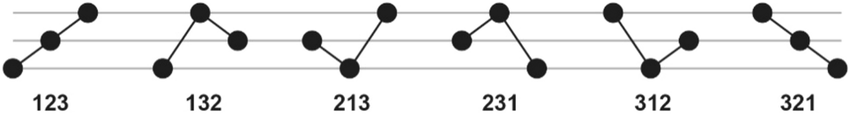
\includegraphics[width=11.81in,]{./fig_1} \caption{The number of possible patterns for the embedding dimension 3}\label{fig:unnamed-chunk-1}
\end{figure}

\section{Methodology}\label{Methodology}

The data are considered from the Bearing data centre and seeded fault
test data at the Case Western Reserve University, School of Engineering.
The data set consists of ball bearing test data for normal bearings,
single-point drive end, and fan end defects. A total of 12,000 and
48,000 data points were considered per second for the drive-end bearing
tests. Fan end bearing was also obtained at a rate of 12,000 data points
per second. Each file includes motor rotational speed, drive end
vibration data, and fan data. For all files, the following item in the
variable name indicates:

\begin{itemize}
  \item DE - drive end accelerometer data
  \item FE - fan end accelerometer data
  \item BA - base accelerometer data
  \item time - time series data
  \item RPM - rpm during testing 
\end{itemize}

Further, for the easiness of use data were separated by the name Normal
Baseline Data, 12k Drive End Bearing Fault Data, 48k Drive End Bearing
Fault Data, and Fan-End Bearing Fault Data. Normal baseline data has
four motor loads 0, 1, 2, and 3. Approximate motor speed was given in
rpm. (1797, 1772, 1750, 1730). 12k Drive End, 48k Drive End and 12k Fan
End bearing data follow the same motor loads and speeds. The research is
conducted to identify the fault machines from the separate time series
data.

Bearings are critical components in rotating machinery, yet their
demanding operating conditions involving high loads and impacts often
lead to various faults. These faults can result in significant downtime,
costly maintenance, and even complete machine failure. Therefore, early
and accurate detection and classification of bearing faults are
essential for ensuring operational reliability and minimizing
maintenance expenses. Traditional fault detection methods primarily rely
on analyzing physical parameters and trends using vibration analysis,
thermal monitoring, and current signature analysis techniques. While
these methods have proven effective, they can be susceptible to noise
and often require substantial computational resources. Ordinal pattern
analysis has emerged as a promising alternative, offering a robust and
computationally efficient approach for analyzing time series data. At
its core, ordinal pattern analysis involves transforming continuous time
series data into a sequence of ordinal patterns that represent the order
relationships among data points within a given time window. This
approach effectively captures the fundamental dynamics of the signal in
a manner that is inherently robust to noise and distortions. By
analyzing these patterns, it becomes possible to identify subtle changes
in system behavior that may indicate the presence of a fault. This study
investigates the application of ordinal pattern analysis for early
detection and classification of bearing faults, focusing on common fault
types such as ball, outer race, and inner race defects. Using a publicly
available dataset from the Case Western Reserve University Bearing Data
Center, we will demonstrate the effectiveness of ordinal patterns in
distinguishing between healthy and faulty bearing conditions. The data
set consist of ball bearing test data for normal bearings, single-point
drive end and fan end defects. A total of 12,000 and 48,000 data points
were considered per second for the drive end bearing tests. Fan end
bearing was also obtained at a rate of 12,000 data points per second.
Each file includes motor rotational speed, drive end vibration data, and
fan data. Further, for the easiness of use data were separated by the
name Normal Baseline Data, 12k Drive End Bearing Fault Data, 48k Drive
End Bearing Fault Data, Fan-End Bearing Fault Data. Normal baseline data
has four motor loads 0, 1, 2, and 3. Approximate motor speed was given
in rpm. (1797, 1772, 1750, 1730). 12k Drive End, 48k Drive End and 12k
Fan End bearing data follows the same motor loads and speeds. The
research is conducted to identify the fault machines. Each data file
consists of two time series and we examined two time series data using
ordinal patterns. We introduce distance as a measure of similarity
between segments based on the ordinal structure. With specific embedding
dimensions, it can be employed to distinguish fault machines. We show an
application of Permutation entropy on rolling bearing fault diagnosis.
The results of this experiment shows that dimension 3 and 4 results
separate fault machines. Some machines recognize with white noise which
is close to the lower and upper boundary. The complexity plane is used
to analyse the results and it has confirmed that dimension 4 is assured
the best results.

Examples of time series data are shown as follows.

\begin{figure}
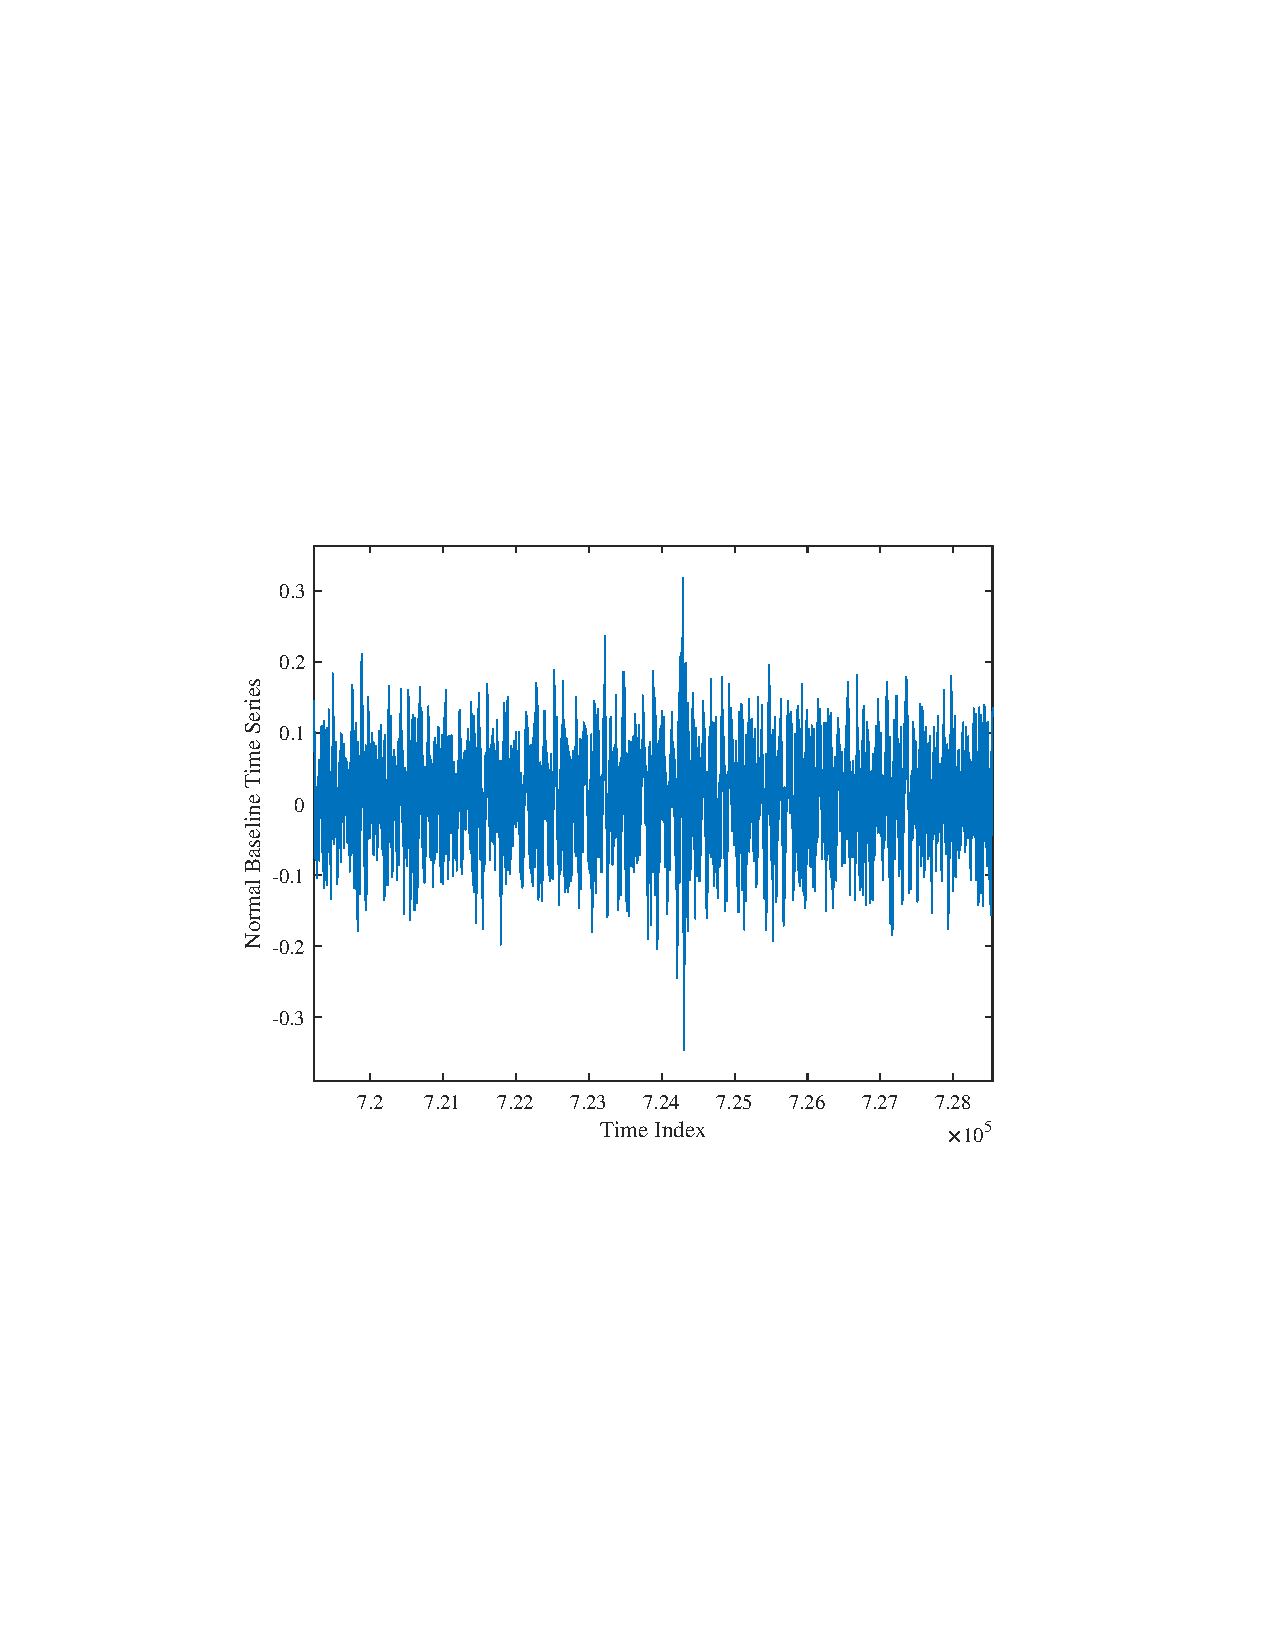
\includegraphics{./normalbaselinetimeSeriesDE} \caption{The number of possible patterns for the embedding dimension 3}\label{fig:unnamed-chunk-2}
\end{figure}

\begin{figure}
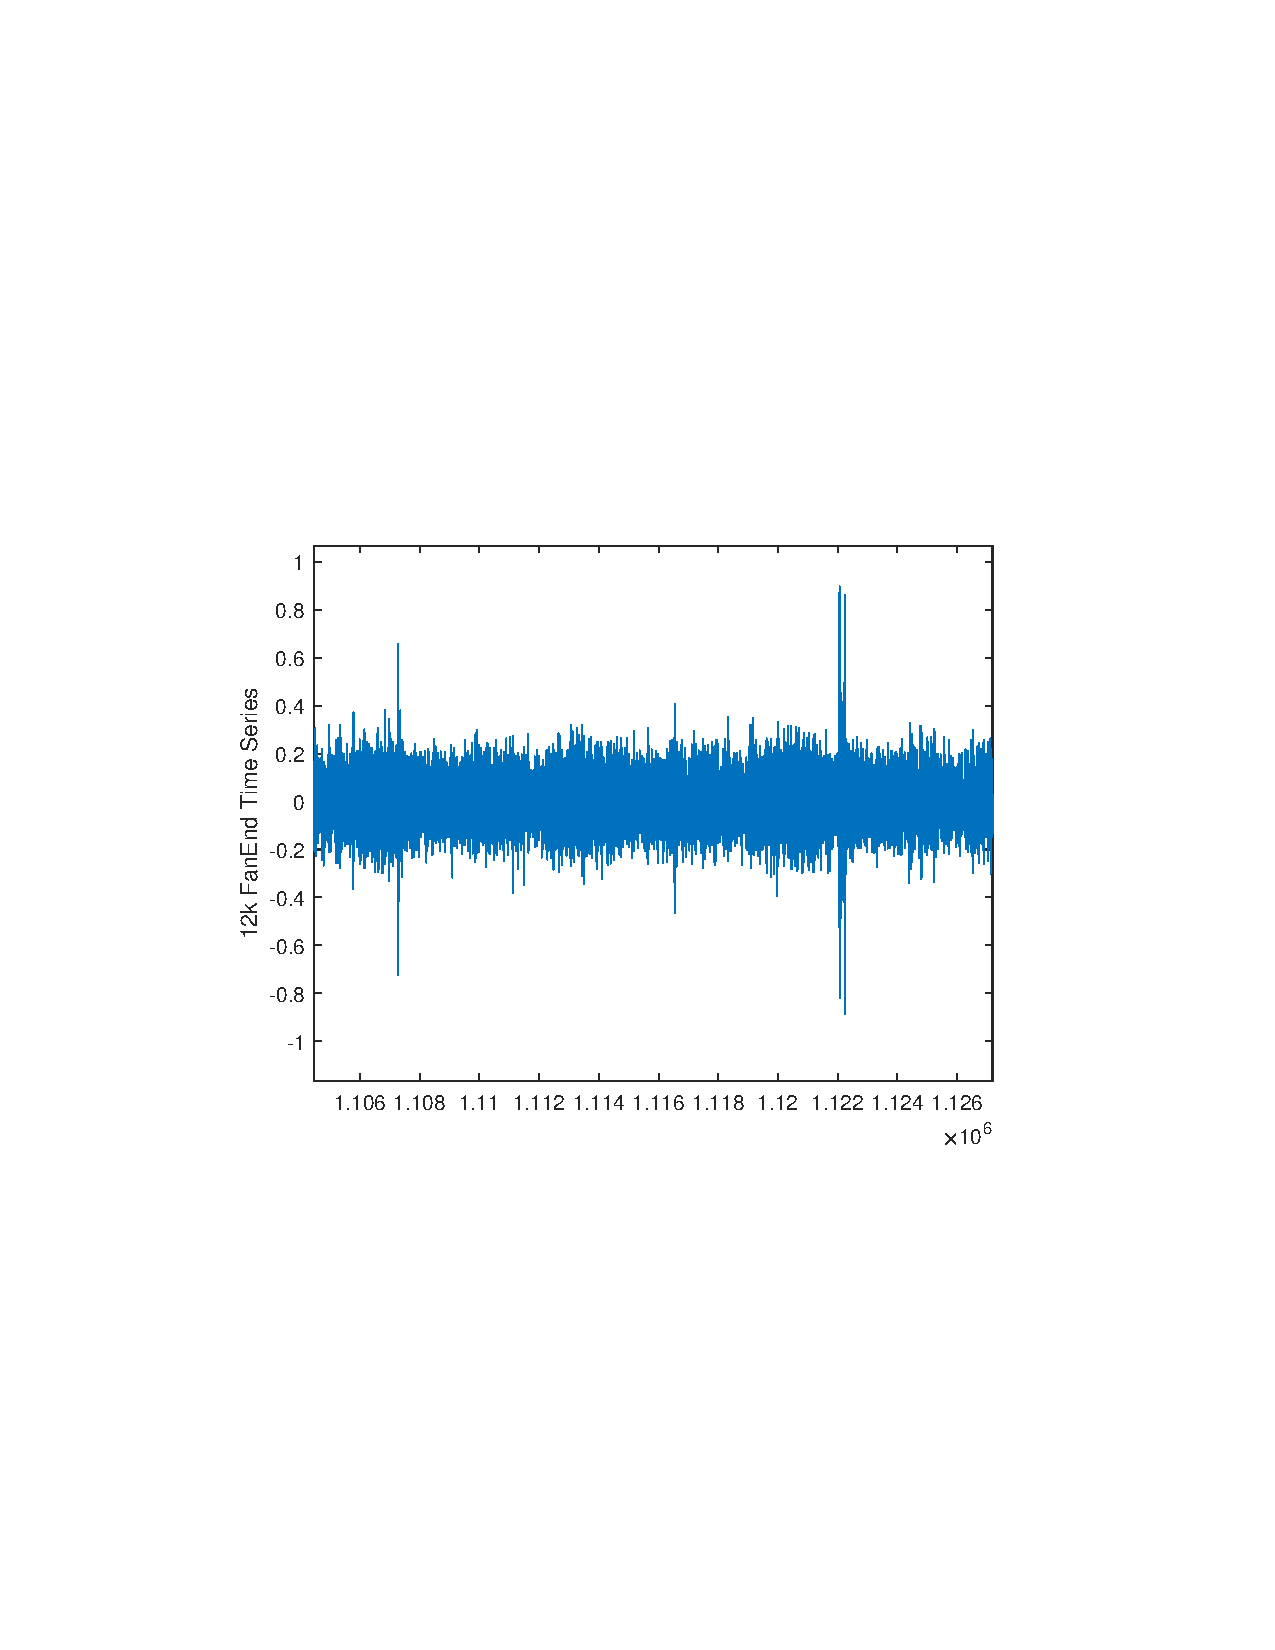
\includegraphics{./fanend12kDE} \caption{The number of possible patterns for the embedding dimension 3}\label{fig:unnamed-chunk-3}
\end{figure}

Figure 2 shows the DE, FE and BA time series for engine loads 0, 1, 2
and 3. Looking at these time series it is not possible to identify the
faulty machines. However, the Figure 3 and 4 shows the normal baseline
DE time series for a motor load of 0 and the accelerometer time series
data at the 12,000 fan end for a motor load of 0. The graph is clear and
it is noticeable that fault time series data consists of time series.
However, it is difficult to separate the exact machine type and other
characteristics of the data. The main idea of this research work is to
identify fault machines from the various time series data given above.
First, time series data was analyzed and then the StatOrdPatt package
introduced by \citet{REY2024115481} was used to analyze the data. Next,
the probability distribution of the ordinal pattern was considered and
the entropy permutation entropy was calculated accordingly. Based on the
entropy of each time series data, the entropy complexity level was
considered to separate the faulty machines.

\section{Results}\label{Results}

The permutation entropy guarantees to separate fault machines. With this
experimental result, we can see that dimensions 3 and 4 result in
separate fault machines. We see that the machines form clusters, but
also that they have individual signatures. The below table shows the
Shannon entropy and the complexity results for embedding dimensions 3
and 4.

\bibliography{BearingFaultDiagnosis.bib}


\end{document}
